\section{Results}
\label{sec:results}

\subsection{E1 -- PHY validation}
The Monte Carlo SER matches the exact noncoherent formula within \EoneMCMaxDiff{} (absolute,
\EoneMCTrials{} trials per point, Fig.~\ref{fig:e1}a). For a 20-byte packet, the ideal receiver reaches
PER\,=\,1\,\% between \EoneGapMax{} and \EoneGapMin{}\,dB from the Semtech thresholds (best margin at
SF12: \EoneGapSFtwelve{}\,dB), so the thresholds are consistent with the model without calibration.

The Doppler rate changes the picture (Fig.~\ref{fig:e1}b). At SNR$_\text{req}$+5\,dB, receiver~A
(no tracking) loses SF12 packets from \CritASFtwelve{}\,Hz/s, SF11 from \CritASFeleven{}\,Hz/s and SF10
from \CritASFten{}\,Hz/s: at the 600\,km zenith rate the payload of an SF12 packet drifts by
\DriftBinsSFtwelve{} bins. Receiver~B (tracking) keeps SF7--SF11 error-free up to 1000\,Hz/s and loses
SF12 between \OkBSFtwelve{} and \CritBSFtwelve{}\,Hz/s, below the noise-free loop limit of
\TrackLimitSFtwelve{}\,Hz/s.

\begin{figure}[t]
\centering
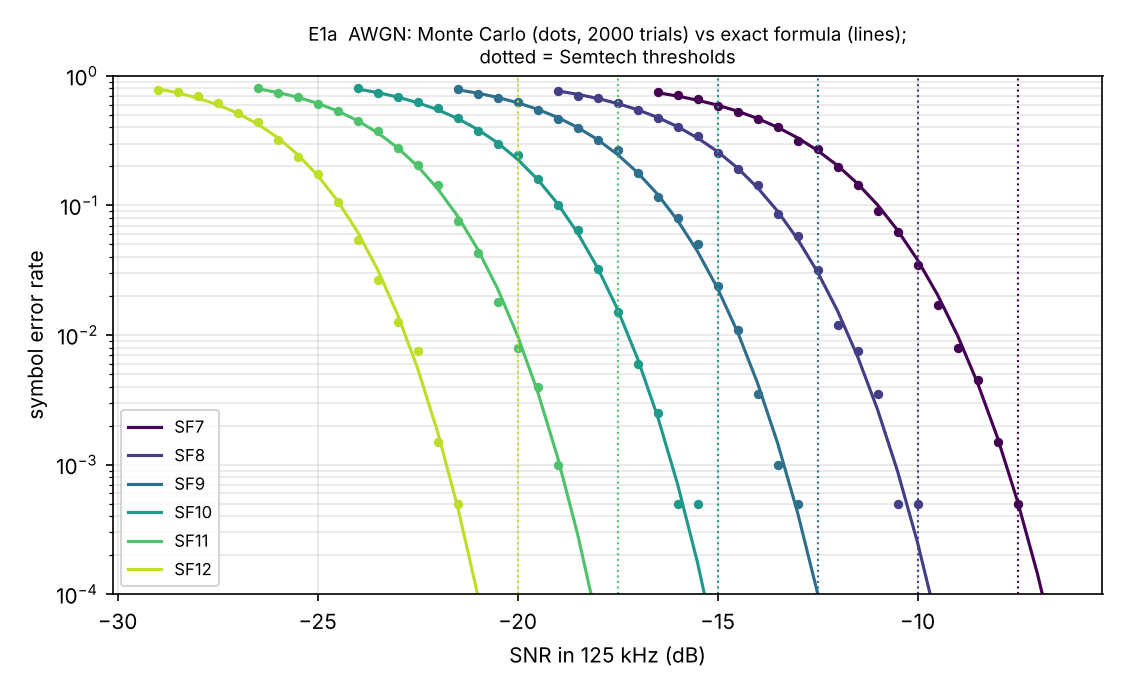
\includegraphics[width=\columnwidth]{../results/e1a_ser_vs_snr_awgn.png}\\[-1mm]
{\small (a)}\\
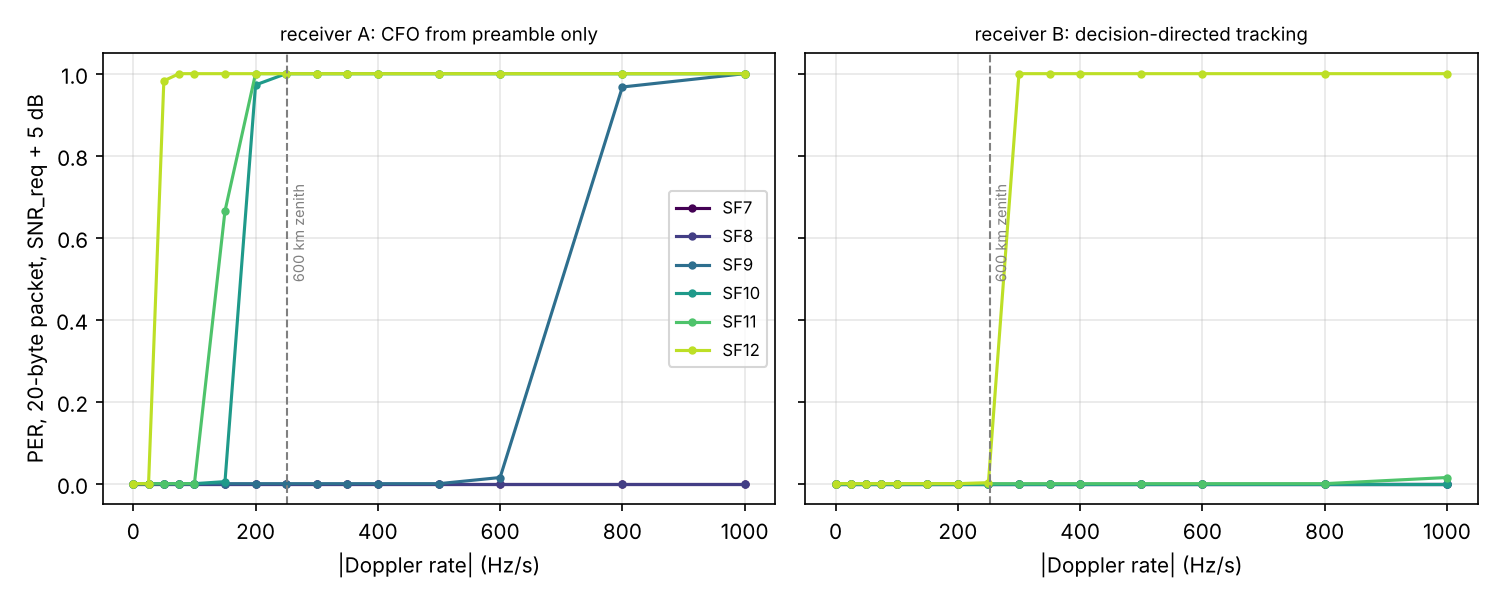
\includegraphics[width=\columnwidth]{../results/e1b_per_vs_doppler.png}\\[-1mm]
{\small (b)}
\caption{E1. (a) SER in AWGN, Monte Carlo (dots) vs exact formula (lines). (b) PER of a 20-byte
packet vs Doppler rate at SNR$_\text{req}$+5\,dB for both receivers.}
\label{fig:e1}
\end{figure}

\subsection{E2 -- Satellite pass}
A 600\,km zenith pass stays above 10$^\circ$ for \EtwoDuration{}\,min, with Doppler up to
$\pm$\EtwoMaxDoppler{}\,kHz, a rate of \EtwoMaxRate{}\,Hz/s at zenith, a one-way delay of
\EtwoDelayMin{}--\EtwoDelayMax{}\,ms and a LOS SNR from \EtwoSnrMin{} to \EtwoSnrMax{}\,dB at 14\,dBm
(Fig.~\ref{fig:e2}). The link only closes at SF$\ge$9 and only near zenith for SF9--10: exactly where the
Doppler rate is highest. With receiver~A, SF12 is usable on \EtwoAshareSFtwelve\,\% of the pass
(\EtwoAshareSFtwelveSnr\,\% if Doppler is ignored): \emph{the most robust SF on the ground is the most
fragile in orbit}, and no single SF is usable over the whole pass: the right SF changes with the
elevation within minutes, far faster than ADR's 20-uplink history. With receiver~B,
SF12 only fails around zenith (usable on \EtwoBshareSFtwelve\,\% of the pass).

The altitude sweep (Fig.~\ref{fig:e2b}) is a check against measurements: with receiver~B, SF12 is
feasible at zenith from \EtwoBSFtwelveZenithFrom\,km upwards (PER $\le$ 1\,\%), while Doroshkin
et al.\ measured SF12 failing near zenith below about 550\,km~\cite{doroshkin2019}, where our zenith
rate is \EtwoRateFiveFifty\,Hz/s. Receiver~B is therefore close to, and slightly more pessimistic than,
real hardware; receiver~A is far too pessimistic. Receiver~B is used in all network experiments.

\begin{figure}[t]
\centering
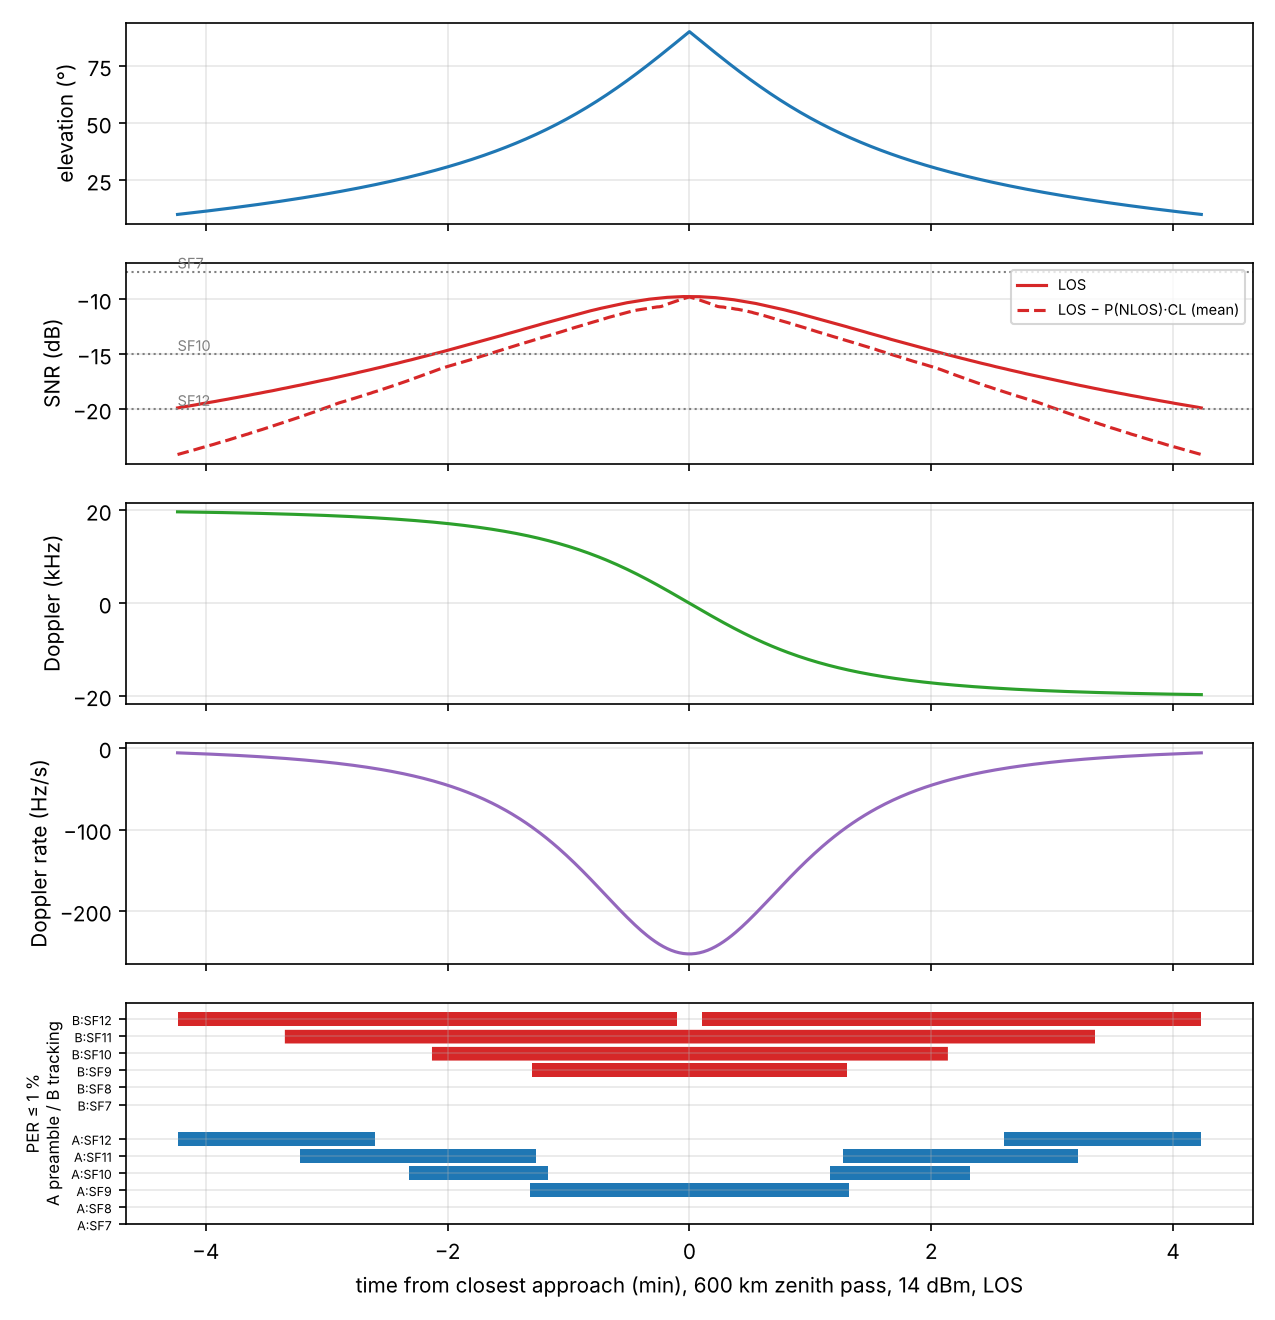
\includegraphics[width=\columnwidth]{../results/e2_satellite_pass.png}
\caption{E2. 600\,km zenith pass: elevation, SNR, Doppler, Doppler rate, and SFs with PER $\le$ 1\,\%
for receivers A and B.}
\label{fig:e2}
\end{figure}

\begin{figure}[t]
\centering
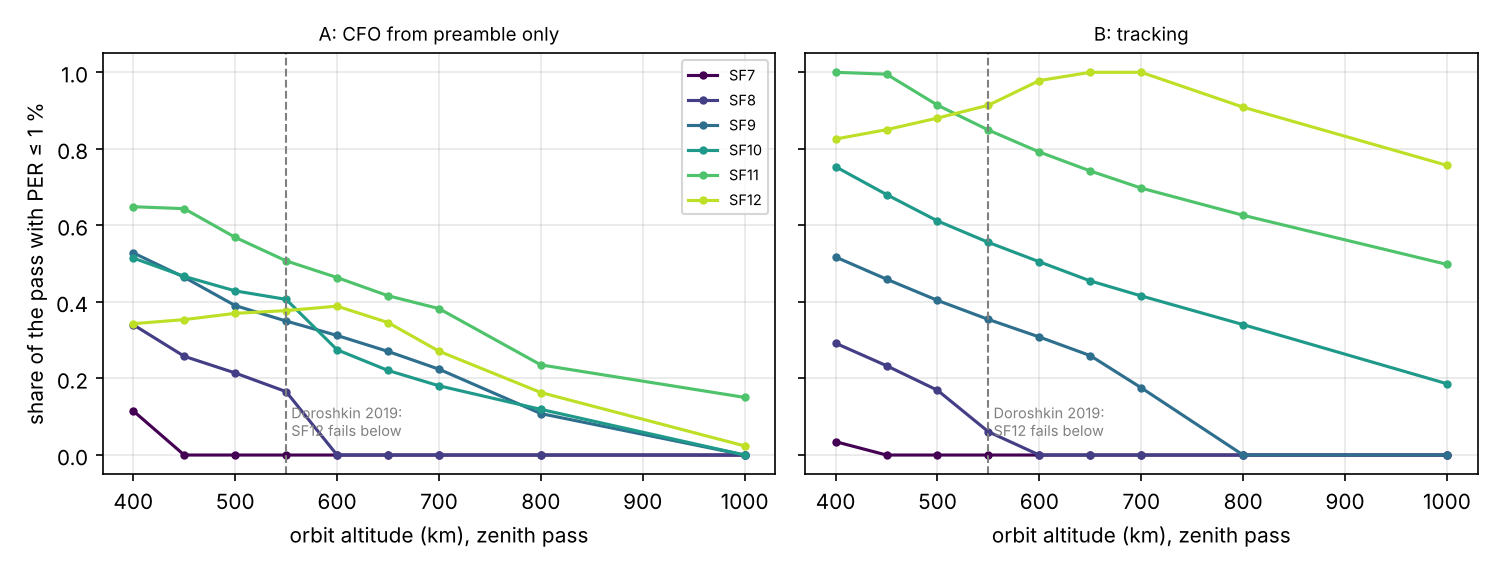
\includegraphics[width=\columnwidth]{../results/e2b_altitude_sweep.png}
\caption{E2b. Share of a zenith pass where each SF reaches PER $\le$ 1\,\%, vs orbit altitude.}
\label{fig:e2b}
\end{figure}

\subsection{E3 -- Scalability without anomalies}
The simulator reproduces pure ALOHA ($|S-Ge^{-2G}|\le$\,\AlohaMaxErr{} up to $G=$\AlohaMaxG{}).
In a terrestrial cell (Fig.~\ref{fig:e3}), ADR delivers \EthreePdrADRLo\,\% of the packets at
$N=\EthreeNlo$ and \EthreePdrADRHi\,\% at $N=\EthreeNhi$, at \EthreeEADRHi\,mJ per delivered packet.
Fixed SF12 collapses with load (\EthreePdrSFtwelveHi\,\% at $N=\EthreeNhi$) because each packet
occupies the channel for 1.3\,s; fixed SF7 stays near \EthreePdrSFsevenHi\,\% because distant devices
cannot reach the gateway. The oracle wins at low load (\EthreePdrOracleLo\,\%) but loses to ADR at
$N=\EthreeNhi$ (\EthreePdrOracleHi\,\%): choosing the lowest energy per packet puts most devices on
SF7 and increases same-SF collisions, while ADR's 10\,dB margin spreads devices over SFs.
The classifier trained on oracle labels under-provisions (\EthreePdrMLHi\,\% at $N=\EthreeNhi$): it
imitates an oracle that knows each packet's fading, and the most likely label given the observable
features is a too-low power or SF. Triggered-Rules is identical to ADR here (no event, no action),
which checks that the triggers stay quiet in normal conditions. The LLM agent equals ADR up to
$N=\EthreeAgentEqualUpTo$ but is below it in \EthreeAgentLossRuns{} of its \EthreeAgentRuns{} runs at
higher load (worst seed \EthreeAgentWorst{} points at $N=\EthreeAgentWorstN$): each time, a false
detector alert coincided with a periodic review and the model moved every device to SF12.

\begin{figure*}[t]
\centering
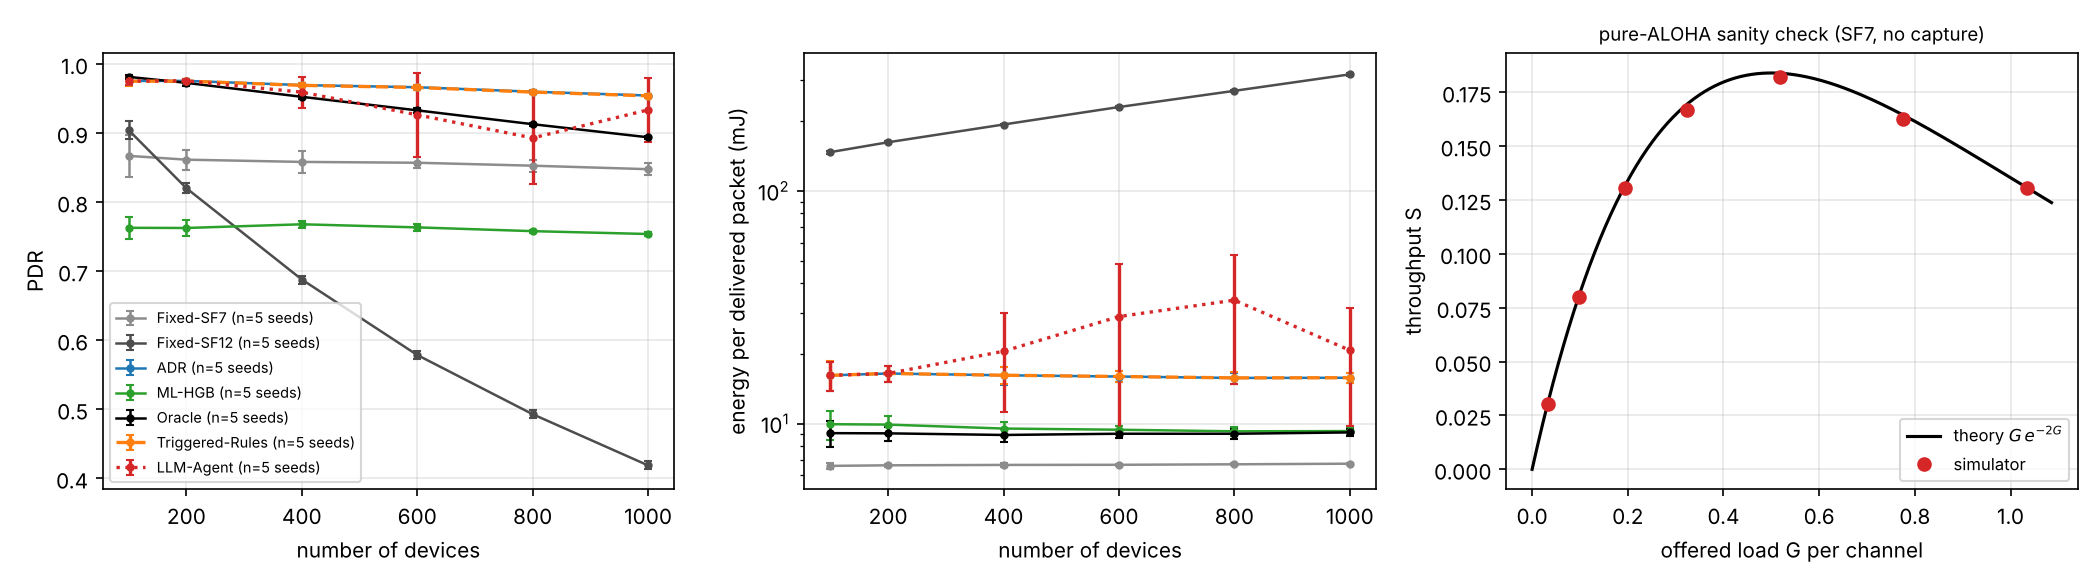
\includegraphics[width=0.95\textwidth]{../results/e3_scalability.png}
\caption{E3. PDR and energy per delivered packet vs number of devices (mean $\pm$ std, 5 seeds), and
the pure-ALOHA check.}
\label{fig:e3}
\end{figure*}
